\section{Introduction}

I remember my first week at a big law firm—honestly, I was shocked by how much time everyone spent just reading contracts. Not analyzing them or making strategic decisions, just reading. Hours and hours of it. My desk neighbor, Sarah, had three banker's boxes of merger documents she'd been working through for two weeks. She told me she'd developed a system: green highlighter for termination clauses, yellow for liability stuff, pink for anything that looked weird. By Friday, those contracts looked like a rainbow threw up on them, and she still wasn't sure she'd caught everything important. That's when it hit me—this can't be the best way to do things in 2024 \cite{katz2017general}.

The legal profession has been crying out for better document review tools for years \cite{zhong2018legal, sulea2017exploring}. When transformer models started making headlines in NLP, many of us thought we'd finally found our answer. But here's the thing—legal documents are beasts of their own. They're incredibly long, stuffed with archaic terminology, and the cost of getting something wrong is astronomical. More importantly, lawyers can't just trust a black box that spits out answers. They need to understand the reasoning behind every decision because they have to defend it in court and explain it to clients who are paying serious money for that advice.

The research community has been making real progress on this front. Take the Contract Understanding Atticus Dataset (CUAD) \cite{hendrycks2021cuad}—over 500 contracts meticulously labeled for 41 different clause types. It's become our go-to benchmark for testing legal AI systems. And then someone had the brilliant idea to actually train a model on legal documents instead of just throwing general-purpose BERT at the problem. Legal-BERT \cite{chalkidis2020legal} was a revelation—suddenly we had a model that actually understood what "whereas" and "heretofore" meant in context, instead of treating them like random vocabulary words. The latest thing that's got me excited is what people are doing with T5 \cite{raffel2020t5} for contract summarization. Imagine being able to feed it a 50-page licensing agreement and getting back a coherent summary that actually captures the important stuff—that would save lawyers like Sarah hours of highlighting.

But we keep running into the same wall: explainability \cite{molnar2020interpretable}. Here's the problem—lawyers don't just need the right answer, they need to be able to explain why it's right. Picture this: you're in a partner meeting and your AI tool flags a clause as potentially problematic. The first question you'll get is "Why?" And "because the algorithm said so" isn't going to cut it. You need to point to specific words, walk through the logic, and convince everyone in that room that you'd bet your bar license on this call. This is where explainable AI methods like SHAP \cite{lundberg2017unified} become essential—they pull back the curtain and show us how these models actually think.

Working with the CUAD dataset has revealed some tough technical challenges that anyone building legal AI needs to grapple with. The first is a brutal class imbalance problem. Only about a third of the possible clauses actually show up in contracts (see Figure \ref{fig:clause_presence_distribution}), which means our models are constantly starved for positive examples. The second challenge is even trickier—clause frequency varies wildly. Every single contract has a "Document Name," but nine clause types appear in fewer than 10\% of contracts (see Figure \ref{fig:clause_presence_frequency}). Finally, these documents are massive. We're talking about an average of nearly 4,800 characters per document (see Figure \ref{fig:context_lengths_distribution}), which pushes even state-of-the-art transformer models to their breaking point \cite{liu2021multilabel}.

\begin{figure}[htbp]
\centering
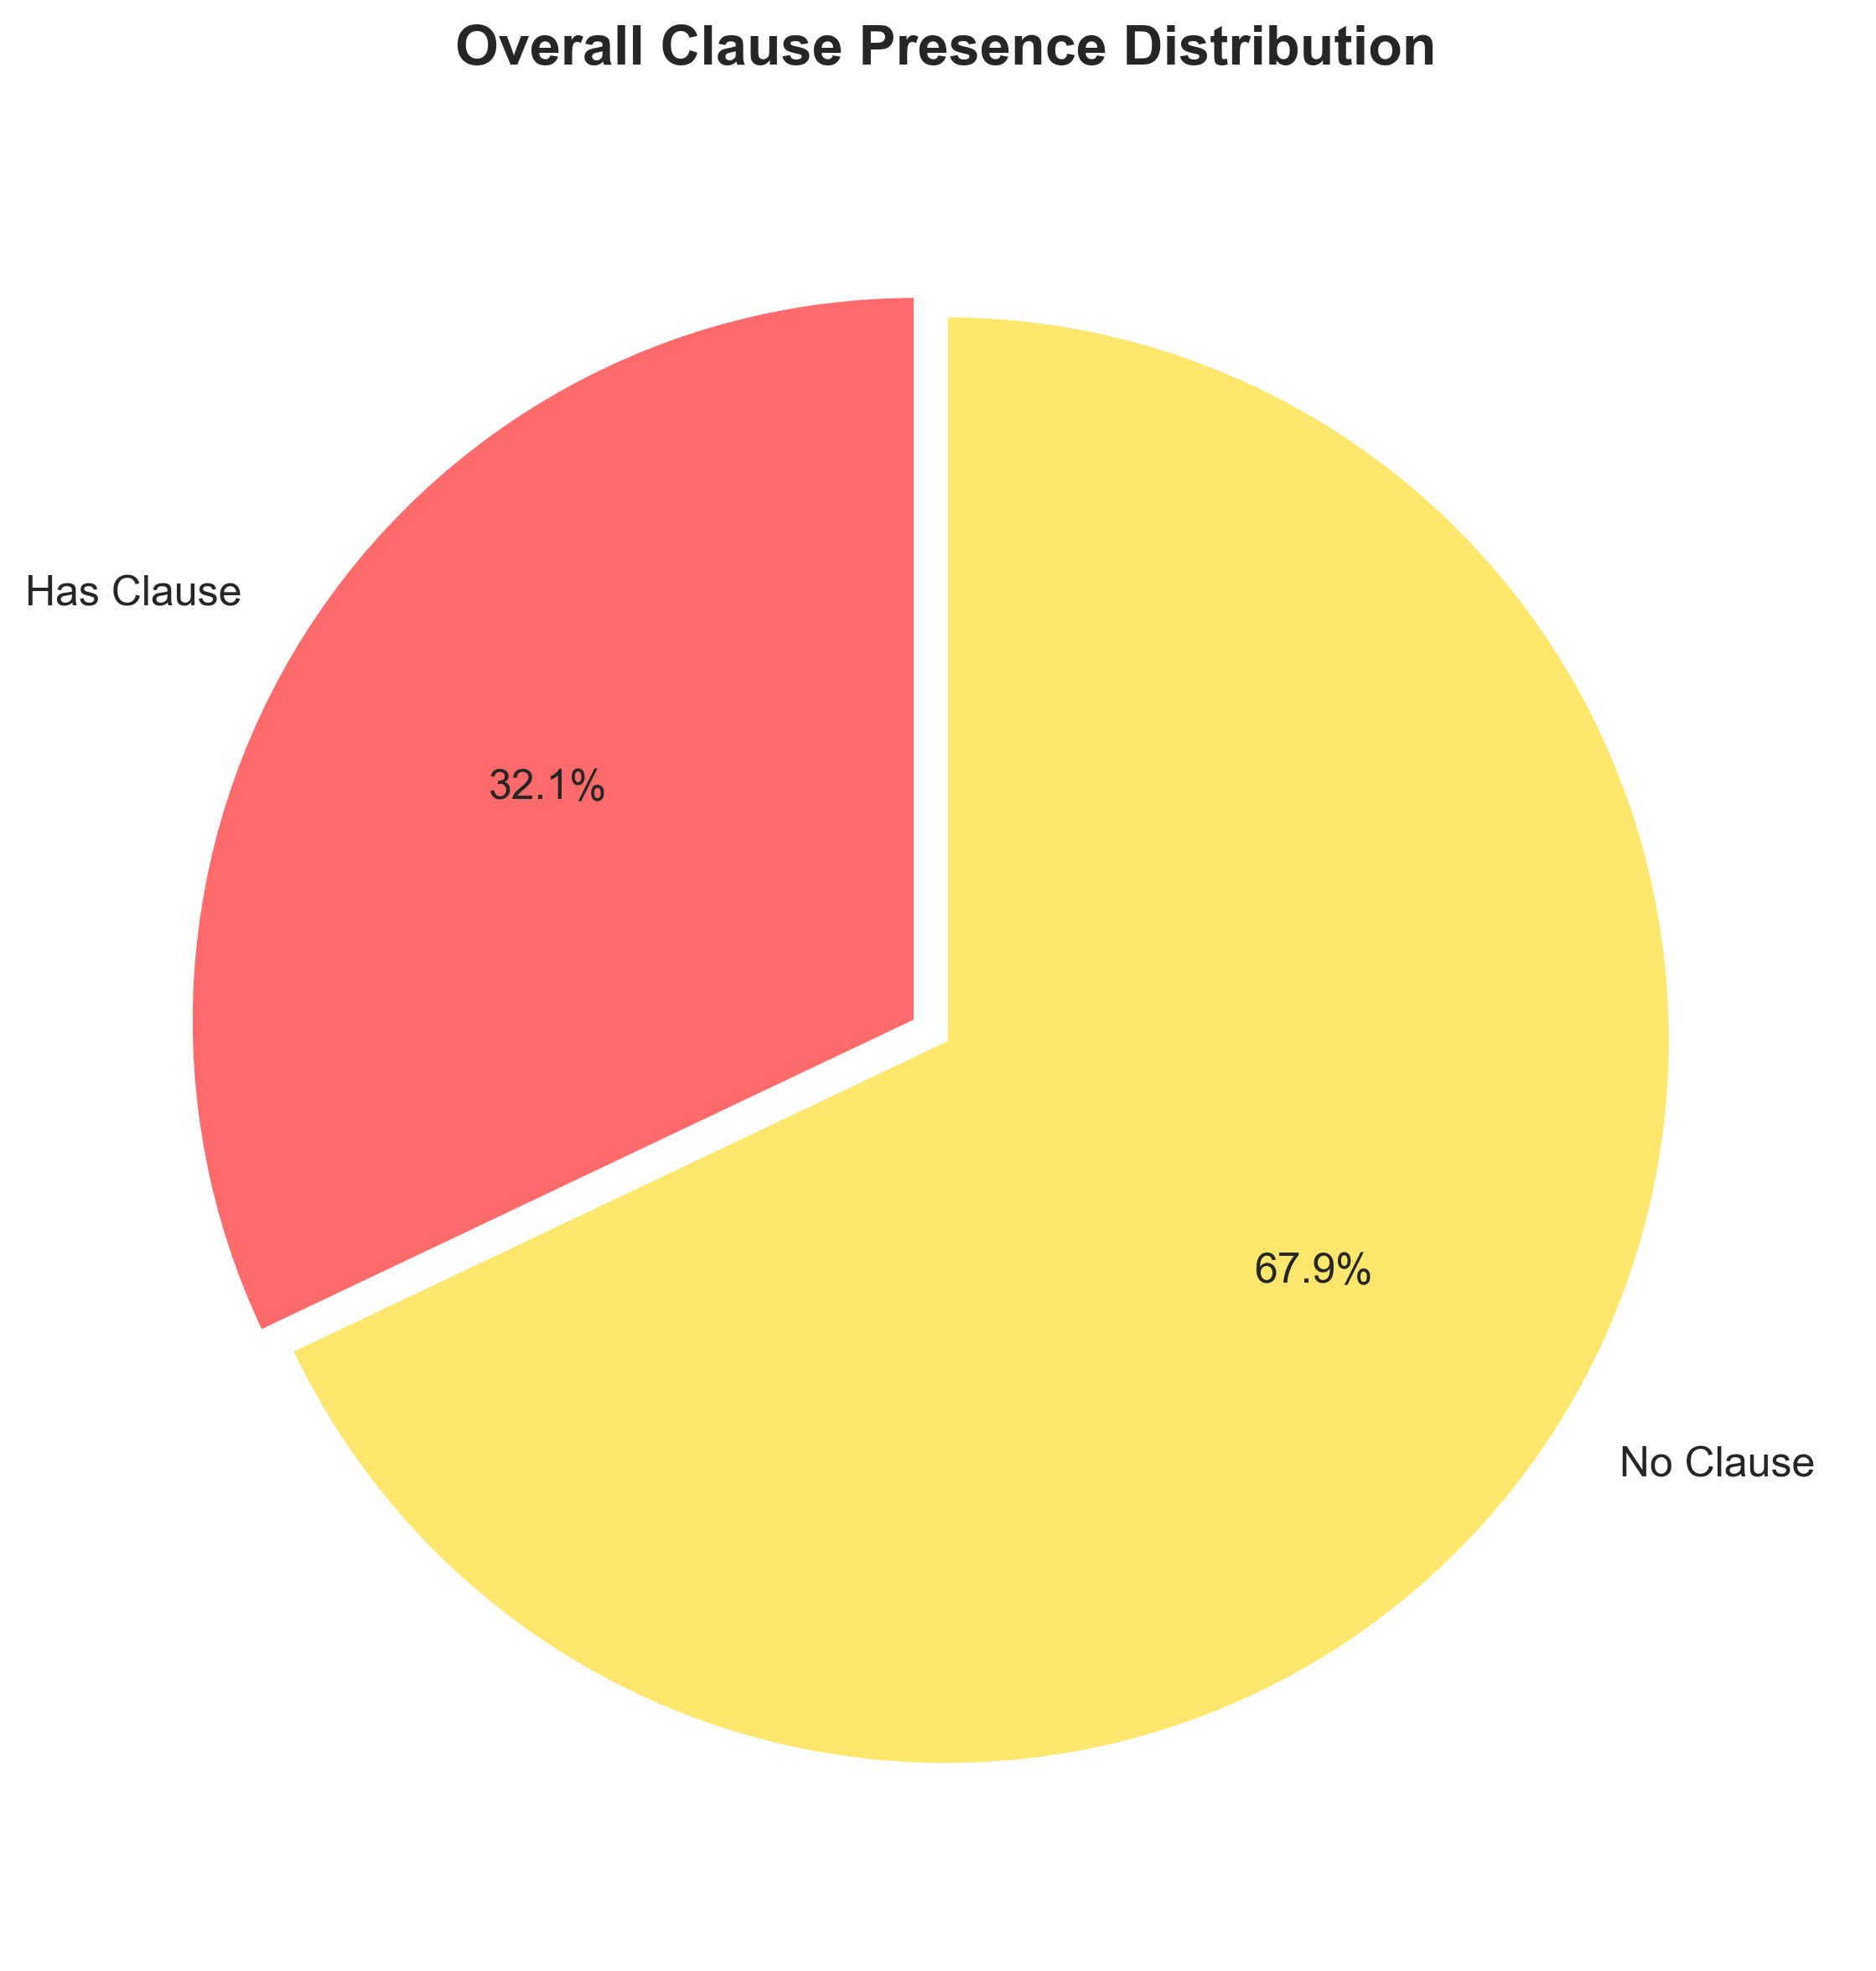
\includegraphics[width=0.45\textwidth]{../figures/clause_presence_distribution.png}
\caption{Overall distribution of clause presence vs. absence in the CUAD dataset, showing severe class imbalance with only 32.1\% positive instances.}
\label{fig:clause_presence_distribution}
\end{figure}

\begin{figure}[htbp]
\centering
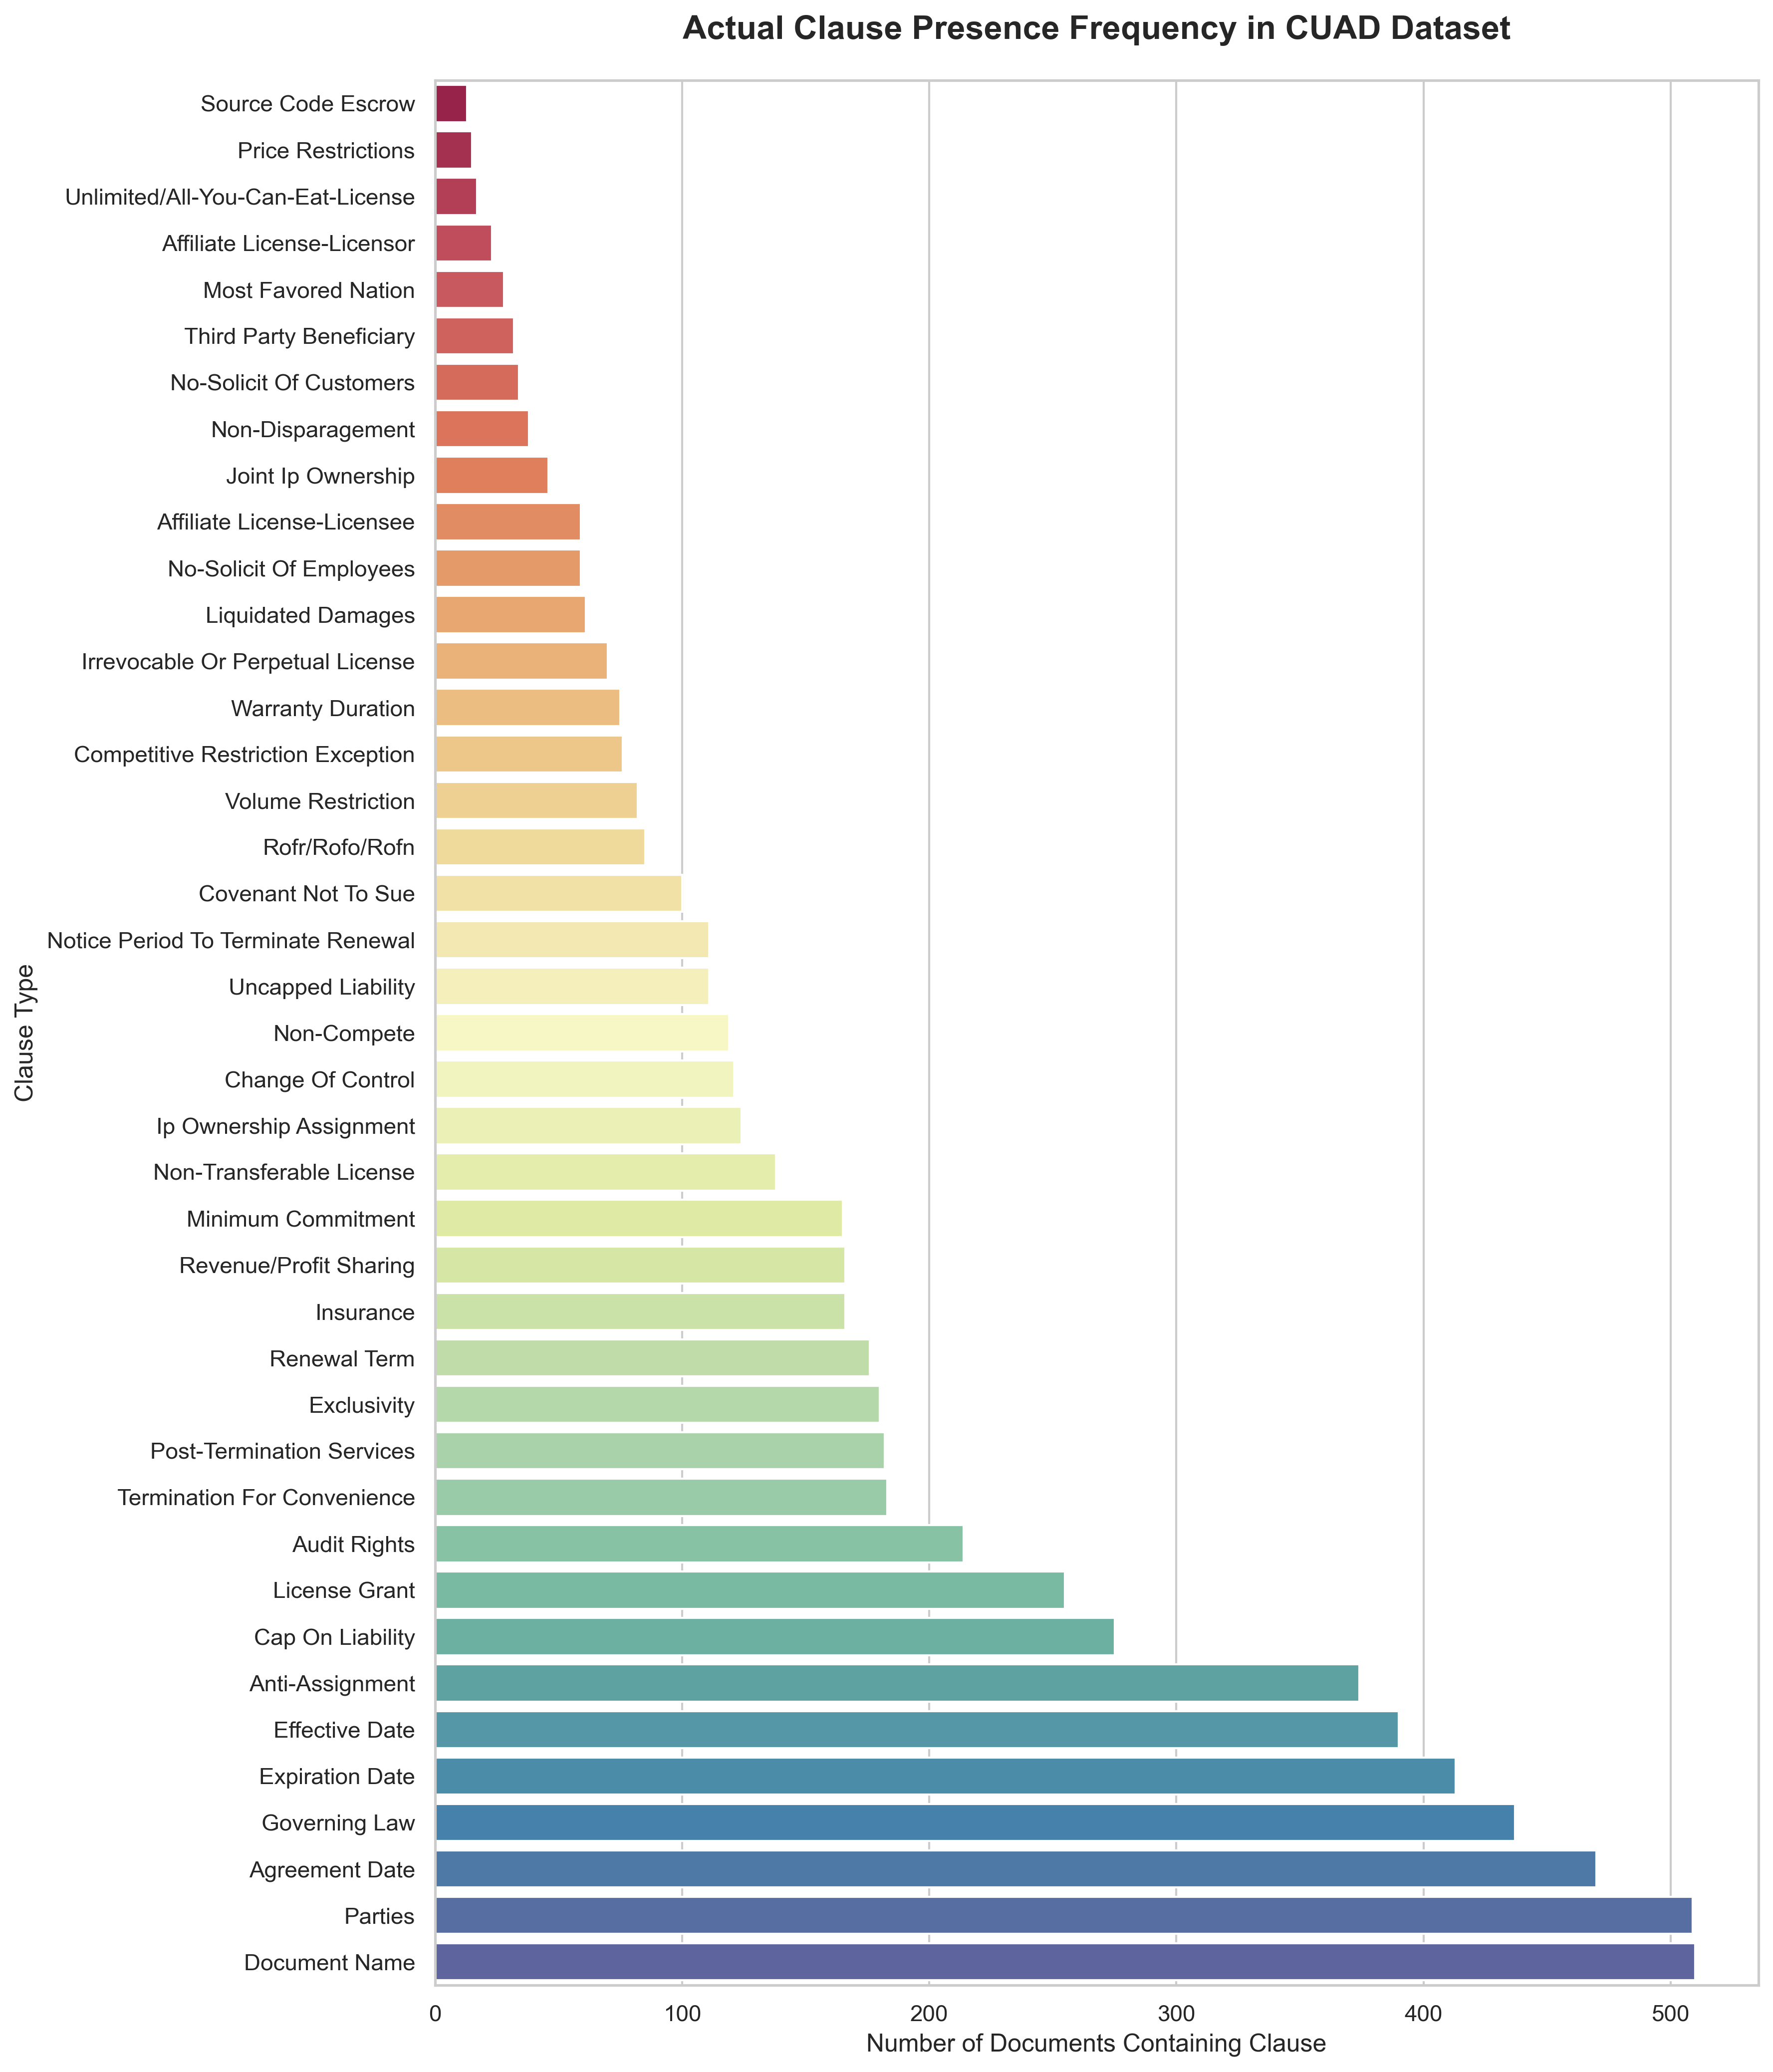
\includegraphics[width=0.48\textwidth]{../figures/clause_presence_frequency.png}
\caption{Frequency distribution of clause types in CUAD dataset, demonstrating extreme variability from universal presence (Document Name) to rare occurrences (\(<10\%\) for nine clause types).}
\label{fig:clause_presence_frequency}
\end{figure}

\begin{figure}[htbp]
\centering
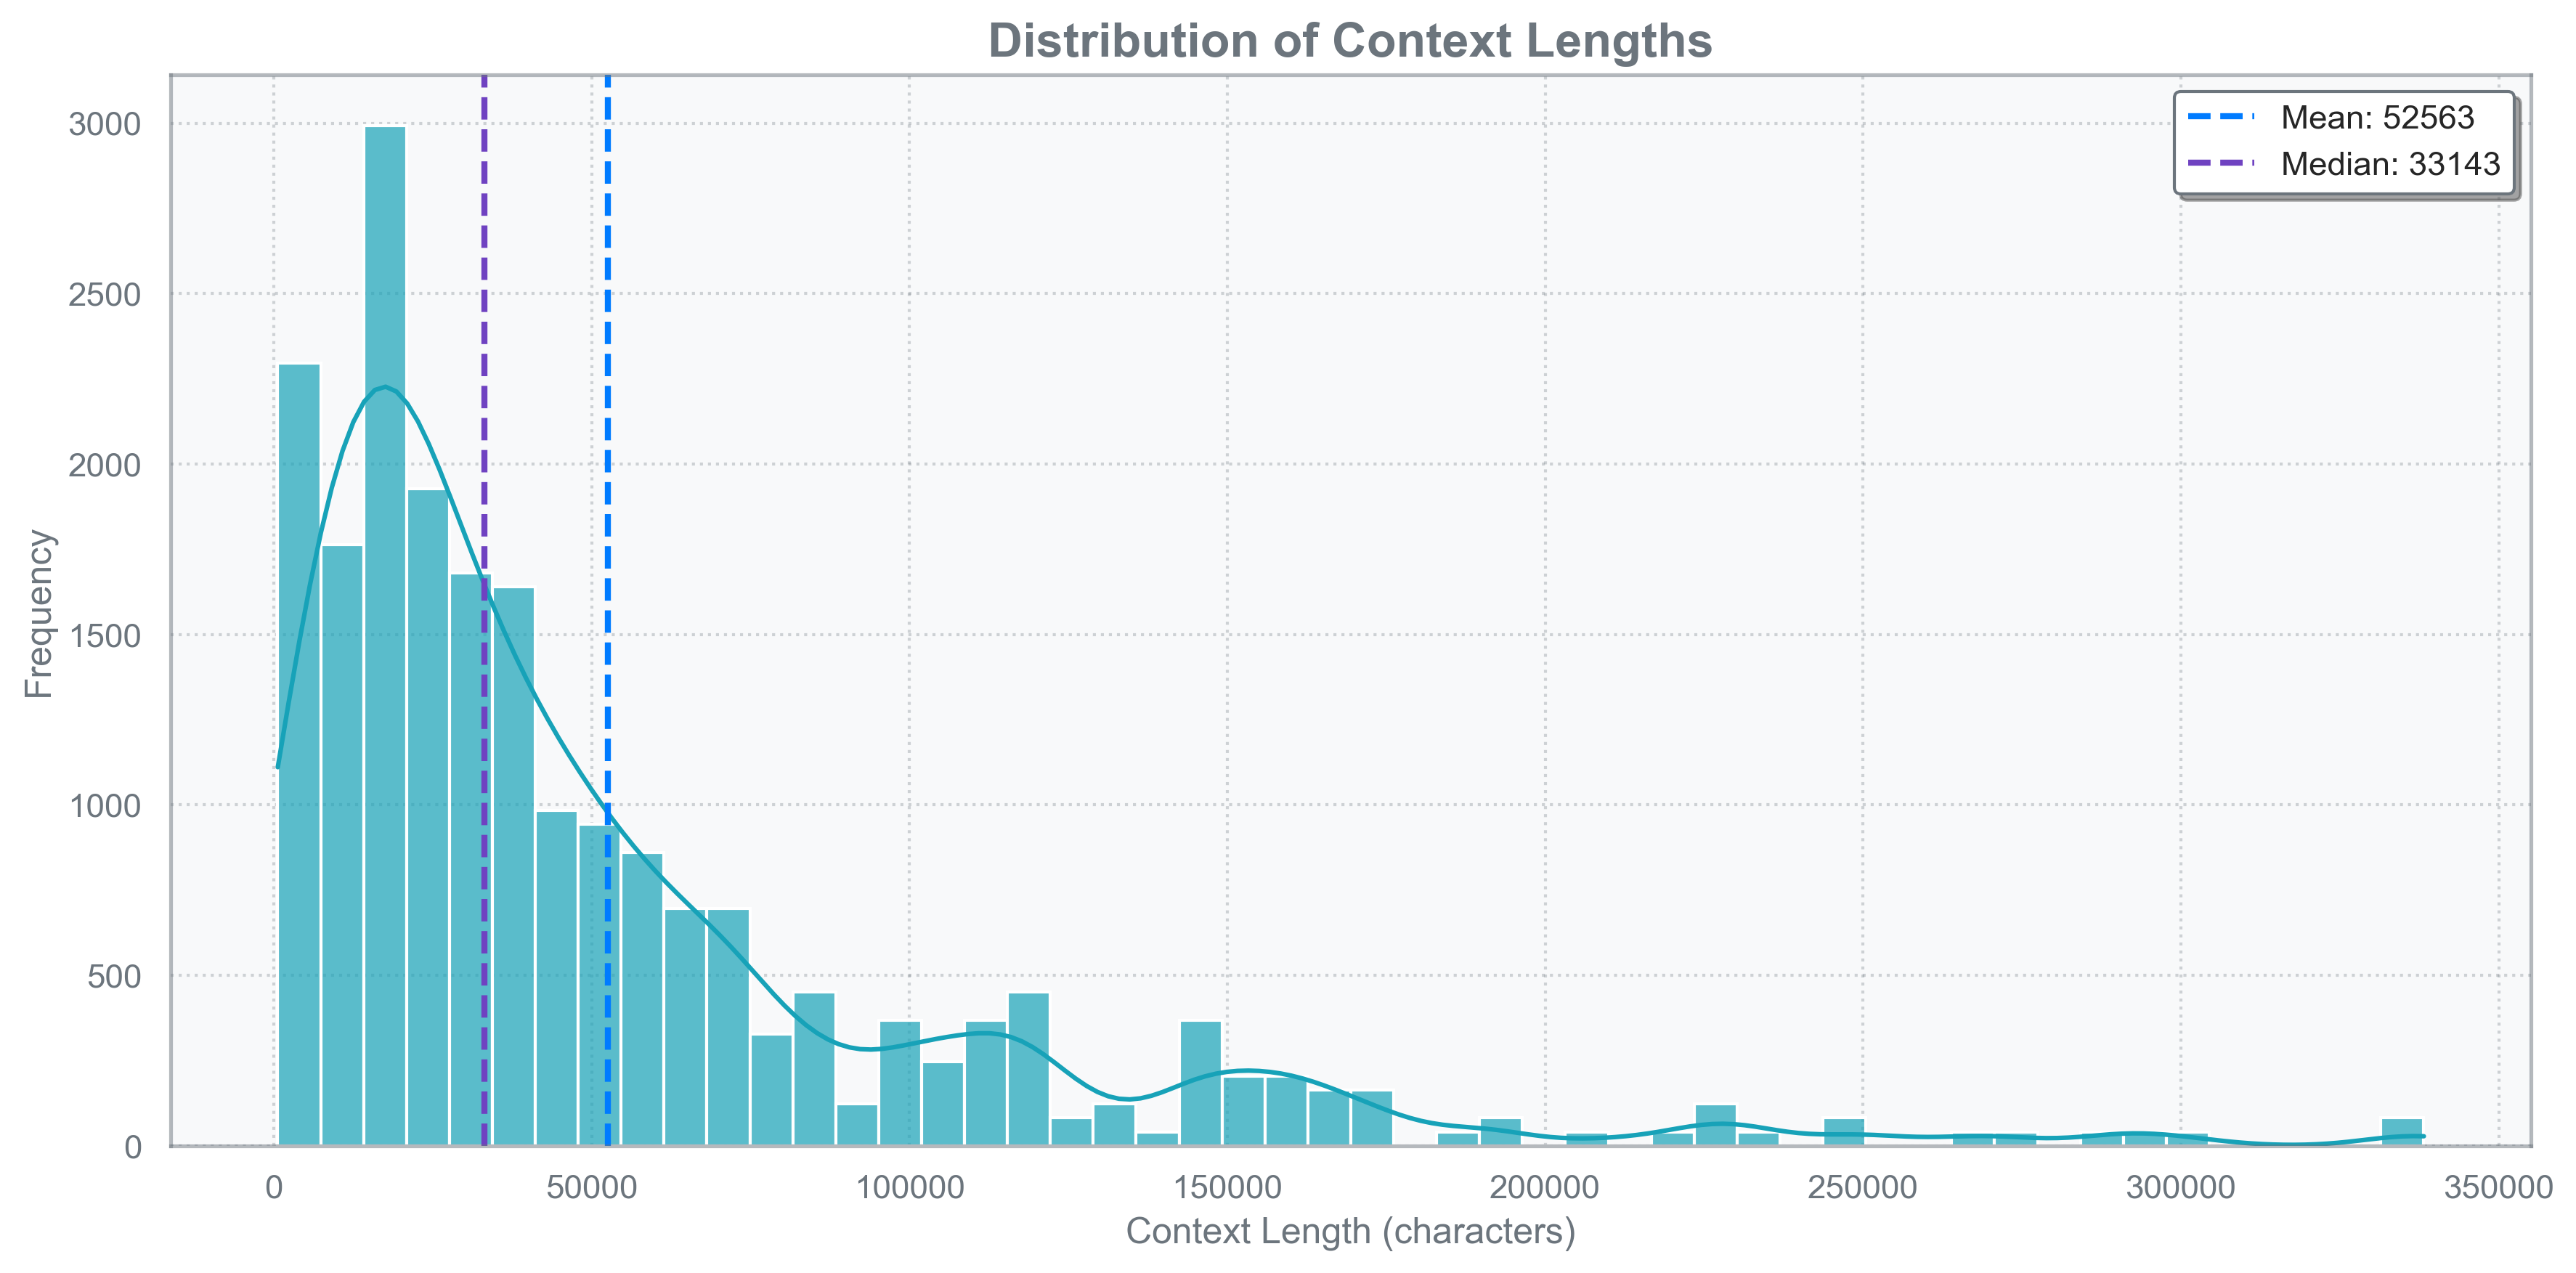
\includegraphics[width=0.45\textwidth]{../figures/context_lengths_distribution.png}
\caption{Distribution of context lengths in legal documents, showing the challenge of processing long sequences with mean length of approximately 4,800 characters.}
\label{fig:context_lengths_distribution}
\end{figure}

The technical challenges are just the beginning. Actually deploying and implementing machine learning in legal practice brings a whole new set of challenges \cite{paleyes2022challenges}. You're dealing with questions of model reliability, data privacy (try explaining to a client why their confidential contract data needs to live in the cloud), regulatory compliance, and somehow fitting all of this into workflows that haven't changed much since the 1980s. In a field where mistakes can cost careers and millions of dollars, these aren't just engineering problems—they're existential questions about the role of AI in the legal system.

But here's the kicker—solving the technical problems is actually the easy part. The real nightmare starts when you try to get this stuff working in an actual law firm \cite{paleyes2022challenges}. I've sat through countless meetings where partners ask questions like "What happens when the model is wrong?" and "How do we know it won't accidentally leak our client's trade secrets?" And don't even get me started on trying to convince a 60-year-old senior partner to change a document review process that's worked the same way since Reagan was president. Trust me, "but the AI is really good" is not a compelling argument when you're talking about client confidentiality and malpractice insurance.

What I present in this paper is my attempt to tackle these challenges head-on. I've built a practical system for interpretable legal document analysis that combines three key components: multi-label clause extraction using BERT models specifically fine-tuned for legal text, abstractive document summarization with T5-based architectures, and comprehensive explainability features using SHAP analysis and attention visualization. The goal was to create something that lawyers could actually use and trust.

I make three main contributions here. First, I've developed a complete end-to-end pipeline that doesn't just identify clauses but explains why it made those decisions. Second, I've conducted a thorough evaluation on the CUAD dataset that reveals exactly how class imbalance affects performance—something that's crucial for understanding when these models can and can't be trusted. Finally, I've wrestled with the practical realities of deploying AI in legal settings and documented what works, what doesn't, and what questions we still need to answer. My hope is that this work helps bridge the gap between the impressive capabilities of modern NLP and the very real, very demanding needs of legal practitioners who are trying to serve their clients better.

